\documentclass{../../oss-apphys}
%\usepackage{bm}

\begin{document}
\genheader

\gentitle{1 \& C}{CIRCULAR MOTION AND SIMPLE HARMONIC MOTION}

\genmultidirections

\gengravity

\raggedcolumns
\begin{multicols}{2}
  \begin{enumerate}[leftmargin=18pt]

  \item Linear acceleration is to force as angular acceleration is to
    \begin{enumerate}[noitemsep,topsep=0pt,leftmargin=18pt,label=(\Alph*)]
    \item kinetic energy
    \item angular velocity
    \item rotational inertia
    \item torque
    \item angular momentum
    \end{enumerate}

  \item A girl stands on a rotating merry-go-round without holding on to a rail.
    The force that keeps her moving in a circle is the
    \begin{enumerate}[noitemsep,topsep=0pt,leftmargin=18pt,label=(\Alph*)]
    \item frictional force on the girl directed away from the center of the
      merry-go-round
    \item frictional force on the girl directed toward the center of the
      merry-go-round
    \item normal force on the girl directed away from the center of the
      merry-go-round
    \item normal force on the girl directed toward the center of the
      merry-go-round
    \item weight of the girl
    \end{enumerate}

    % This problem needs some fixing. None of the answers are correct
%  \item A \SI{.5}{\kilo\gram} ball on the end of a \SI{.5}{\metre} long string
%    is swung in a horizontal circle. What would the speed of the ball have to
%    be for the tension in the string to be \SI{9.}{\newton}?
%    \begin{center}
%      \vspace{-.1in}
%      \pic{.4}{ball-horizontal1.png}
%    \end{center}
%    \begin{enumerate}[noitemsep,topsep=0pt,leftmargin=18pt,label=(\Alph*)]
%    \item\SI{1}{\metre\per\second}
%    \item\SI{3}{\metre\per\second}
%    \item\SI{6}{\metre\per\second}
%    \item\SI{9}{\metre\per\second}
%    \item\SI{12}{\metre\per\second}
%    \end{enumerate}
    
  \item A ball of mass $m$ is swung in a vertical circle of radius $R$. The
    speed of the ball at the bottom of the circle is $v$. The tension in the
    string at the bottom of the circle is
    \begin{enumerate}[noitemsep,topsep=0pt,leftmargin=18pt,label=(\Alph*)]
    \item $\displaystyle mg$
    \item $\displaystyle mg+\frac{mv^2}{R}$
    \item $\displaystyle mg-\frac{mv^2}{R}$
    \item $\displaystyle \frac{mv^2}{R}$
    \item zero
    \end{enumerate}
    \columnbreak
    
  \item A car of mass $m$ drives on a flat circular track of radius $R$. To
    maintain a constant speed $v$ on the track, the coefficient of friction
    $\mu$ between the tires and the road must be
    \begin{enumerate}[noitemsep,topsep=0pt,leftmargin=18pt,label=(\Alph*)]
    \item $\displaystyle mg$
    \item $\displaystyle mg+\frac{mv^2}{R}$
    \item $\displaystyle mg-\frac{mv^2}{R}$
    \item $\displaystyle \frac{v^2}{gR}$
    \item $\displaystyle \sqrt{\frac{v^2}{gR}}$
    \end{enumerate}
    
  \item A meter stick of mass \SI{.1}{\kilo\gram} rests on a table as shown. A
    length of \SI{40}{\centi\metre} extends over the edge of the table. How far
    from the edge of the table could a \SI{.05}{\kilo\gram} mass be placed on
    the meter stick so that the stick just begins to tip?
    \begin{center}
      \vspace{-.2in}
      \pic{.3}{beam1.png}
    \end{center}
    \begin{enumerate}[noitemsep,topsep=0pt,leftmargin=18pt,label=(\Alph*)]
    \item\SI{5}{\centi\metre}
    \item\SI{10}{\centi\metre}
    \item\SI{15}{\centi\metre}
    \item\SI{20}{\centi\metre}
    \item\SI{30}{\centi\metre}
    \end{enumerate}
    \columnbreak
    
  \item A meter stick is balanced on a fulcrum at its center, as shown. A mass
    of \SI{5}{\kilo\gram} is hung on the left end of the stick, and a mass of
    \SI{2}{\kilo\gram} is hung on the right end. In order to balance the
    system, a mass $m$ is hung at the $25$-\si{\centi\metre} mark on the right
    side. What is the value of the mass $m$?
    \begin{center}
      \pic{.35}{beam2.png}
    \end{center}
    \begin{enumerate}[noitemsep,topsep=0pt,leftmargin=18pt,label=(\Alph*)]
    \item\SI{12}{\kilo\gram}
    \item\SI{6 }{\kilo\gram}
    \item\SI{4 }{\kilo\gram}
    \item\SI{3 }{\kilo\gram}
    \item\SI{2 }{\kilo\gram}
    \end{enumerate}
    
  \item A ball on the end of a string is swung in a circle of radius
    \SI{2}{\metre} according to the equation $\theta = 4t^2+3t$, where $\theta$
    is in radians and $t$ is in seconds. The angular acceleration of the ball
    is
    \begin{enumerate}[noitemsep,topsep=0pt,leftmargin=18pt,label=(\Alph*)]
    \item\SI{6}{rad\per\second^2}
    \item $4t^2 + 3t$ \si{rad\per\second^2}
    \item $8t +3$ \si{rad\per\second^2}
    \item $\displaystyle\frac{3}{4} t^3 + 3t^2$ \si{rad\per\second^2}
    \item \SI{8}{rad\per\second^2}
    \end{enumerate}
  
  \item The linear speed $v$ of the ball (in the previous question) at
    $t=\SI{3}{\second}$ is
    \begin{enumerate}[noitemsep,topsep=0pt,leftmargin=18pt,label=(\Alph*)]
    \item\SI{27 }{\metre\per\second}
    \item\SI{54 }{\metre\per\second}
    \item\SI{108}{\metre\per\second}
    \item\SI{135}{\metre\per\second}
    \item\SI{210}{\metre\per\second}
    \end{enumerate}
    \columnbreak
    
  \item A metal bar of constant density and weight $W$ is attached to a pivot on
    the wall at point $P$ and supported by a rope that makes an angle of
    \ang{60} with the vertical wall. The reaction force exerted by the pivot on
    the bar at point P is best represented by which arrow?
    \begin{center}
      \pic{.25}{metal-bar.png}
    \end{center}
    \begin{enumerate}[noitemsep,topsep=0pt,leftmargin=18pt,label=(\Alph*)]
    \item\vspace{-.15in} $\nearrow$
    \item $\uparrow$
    \item $\downarrow$
    \item $\nwarrow$
    \item $\searrow$
    \end{enumerate}

  \item A uniform rod of length $L$ and mass $m$ has a rotational inertia of
    $\displaystyle \frac{1}{12}mL^2$ about its center. A particle, also of mass
    $m$, is attached to one end of the stick. The combined rotational inertia of
    the stick and particle about the center of the rod is
    \begin{center}
      \pic{.3}{I.png}
    \end{center}
    \begin{enumerate}[noitemsep,topsep=0pt,leftmargin=18pt,label=(\Alph*)]
    \item$\displaystyle\frac{mL^2}{3}$
    \item$\displaystyle\frac{12mL^2}{13}$
    \item$\displaystyle\frac{13mL^2}{12}$
    \item$\displaystyle\frac{mL^2}{156}$
    \item$\displaystyle\frac{13mL^2}{156}$
    \end{enumerate}
    \columnbreak
    
  \item A hoop of radius $R$ and mass $m$ has a rotational inertia of $mR^2$.
    The hoop rolls without slipping along a horizontal floor with a constant
    speed $v$ and then rolls up a long incline. The hoop can roll up the
    incline to a maximum vertical height of
    \begin{center}
      \pic{.4}{hoop1.png}
    \end{center}
    \begin{enumerate}[noitemsep,topsep=0pt,leftmargin=18pt,label=(\Alph*)]
    \item$\displaystyle\frac{v^2}{g}$
    \item$\displaystyle\frac{2v^2}{g}$
    \item$\displaystyle\frac{v^2}{2g}$
    \item$\displaystyle\frac{4v^2}{g}$
    \item$\displaystyle\frac{v^2}{4g}$
    \end{enumerate}
    
  \item Two disks are fixed to a vertical axle that is rotating with a constant
    angular speed $\omega$. The smaller disk has a mass $m$ and a radius $r$,
    and the larger disk has a mass $2m$ and radius $2r$. The general equation
    for the rotational inertia of a disk of mass $M$ and radius $R$ is
    $\frac{1}{2}MR^2$. The ratio of the angular momentum of the larger disk to
    the smaller disk is
    \begin{center}
      \pic{.25}{2disks.png}
    \end{center}
    \begin{enumerate}[noitemsep,topsep=0pt,leftmargin=18pt,label=(\Alph*)]
    \item$1:4$
    \item$4:1$
    \item$1:2$
    \item$2:1$
    \item$8:1$
    \end{enumerate}
    \columnbreak
    
  \item A light rod has a mass attached at each end. At one end is a
    \SI{6}{\kilo\gram} mass, and at the other end is a \SI{3}{\kilo\gram} mass.
    An axis can be placed at any of the points shown. Through which point
    should an axis be placed so that the rotational inertia is the greatest
    about that axis?
    \begin{center}
      \pic{.4}{light-rod.png}
    \end{center}
    \begin{enumerate}[noitemsep,topsep=0pt,leftmargin=18pt,label=(\Alph*)]
    \item A
    \item B
    \item C
    \item D
    \item E
    \end{enumerate}
    
  \item Two wheels are attached to each other and fixed so that they can only
    turn together. The smaller wheel has a radius of $r$ and the larger wheel
    has a radius of $3r$. The two wheels can rotate together on a frictionless
    axle. Three forces act tangentially on the edge of the wheels as shown.
    The magnitude of the net torque acting on the system of wheels is
    \begin{center}
      \pic{.25}{2wheels.png}
    \end{center}
    \begin{enumerate}[noitemsep,topsep=0pt,leftmargin=18pt,label=(\Alph*)]
    \item$Fr$
    \item$2Fr$
    \item$3Fr$
    \item$4Fr$
    \item$6Fr$
    \end{enumerate}
    \columnbreak
    
  \item Astronauts are conducting an experiment in a negligible gravity
    environment. Two spheres of mass m are attached to either end of a light
    rod. As the rod and spheres float motionless in space, an astronaut
    launches a piece of sticky clay, also of mass m, toward one of the spheres
    so that the clay strikes and sticks to the sphere perpendicular to the rod.
    Which of the following statements is true of the motion of the rod, clay,
    and spheres after the collision?
    \begin{center}
      \pic{.25}{collision1.png}
    \end{center}
    \begin{enumerate}[noitemsep,topsep=0pt,leftmargin=18pt,label=(\Alph*)]
    \item Linear momentum is not conserved, but angular momentum is conserved.
    \item Angular momentum is not conserved, but linear momentum is conserved.
    \item Kinetic energy is conserved, but angular momentum is not conserved.
    \item Kinetic energy is conserved, but linear momentum is not conserved.
    \item Both linear momentum and angular momentum are conserved, but kinetic
      energy is not conserved.
    \end{enumerate}

  \item A belt is wrapped around two wheels as shown. The smaller wheel has
    a radius $r$, and the larger wheel has a radius $2r$. When the wheels turn,
    the belt does not slip on the wheels, and gives the smaller wheel an
    angular speed $\omega$. The angular speed of the larger wheel is
    \begin{center}
      \pic{.3}{wheels.png}
    \end{center}
    \begin{enumerate}[noitemsep,topsep=0pt,leftmargin=18pt,label=(\Alph*)]
    \item $\displaystyle \omega$
    \item $\displaystyle 2\omega$
    \item $\displaystyle \frac{1}{2}\omega$
    \item $\displaystyle \frac{1}{4}\omega$
    \item $\displaystyle 4\omega$
    \end{enumerate}
    \columnbreak


  \item One end of a stick of length $L$, rotational inertia $I$, and mass $m$
    is pivoted on an axle with negligible friction at point $P$. The other end
    is tied to a string and held in a horizontal position. When the string is
    cut, the stick rotates counterclockwise. The angular speed $\omega$ of the
    stick when it reaches the bottom of its swing is
    \begin{center}
      \pic{.4}{end-of-stick.png}
    \end{center}
    \begin{enumerate}[noitemsep,topsep=0pt,leftmargin=18pt,label=(\Alph*)]
    \item$\displaystyle\frac{mgL}{I}$
    \item$\displaystyle\sqrt{\frac{mgL}{I}}$
    \item$\displaystyle\sqrt{\frac{2mgL}{I}}$
    \item$\displaystyle\sqrt{\frac{mgL}{2I}}$
    \item$\displaystyle\sqrt{\frac{4mgL}{I}}$
    \end{enumerate}

  \item A disk is mounted on a fixed axle. The rotational inertia of the disk is
    $I$. The angular velocity of the disk is decreased from $\omega_0$ to
    $\omega_f$ during a time $\Delta t$ due to friction in the axle. The
    magnitude of the average net torque acting on the wheel is
    \begin{enumerate}[noitemsep,topsep=0pt,leftmargin=18pt,label=(\Alph*)]
    \item $\displaystyle\frac{\omega_f-\omega_0}{\Delta t}$
    \item $\displaystyle\frac{(\omega_f-\omega_o)^2}{\Delta t}$
    \item $\displaystyle\frac{I(\omega_f-\omega_o)}{\Delta t}$
    \item $\displaystyle\frac{I(\omega_f-\omega_o)^2}{\Delta t}$
    \item $\displaystyle\frac{I(\omega_f-\omega_o)}{\Delta t^2}$
    \end{enumerate}
    \columnbreak
    
  \item The average power developed by the friction in the axle of the disk
    from the previous question to bring it to a complete stop is
    \begin{enumerate}[noitemsep,topsep=0pt,leftmargin=18pt,label=(\Alph*)]
    \item $\displaystyle\frac{\omega_o}{\Delta t}$
    \item $\displaystyle\frac{(\omega_o)^2}{\Delta t}$
    \item $\displaystyle\frac{I(\omega_f-\omega_o)}{2\Delta t}$
    \item $\displaystyle\frac{I\omega_o^2}{2\Delta t}$
    \item $\displaystyle\frac{I(\omega_f-\omega_o)}{\Delta t^2}$
    \end{enumerate}
    
  \item A light rod of negligible mass is pivoted at point $P$ a distance $L$
    from one end as shown. A mass $m$ is attached to the left end of the rod at
    a distance of $3L$ from the pivot, and another mass $4m$ is attached to the
    other end a distance $L$ from the pivot. The system begins from rest in the
    horizontal position. The net torque acting on the system due to
    gravitational forces is
    \begin{center}
      \pic{.4}{light-rod2.png}
    \end{center}
    \begin{enumerate}[noitemsep,topsep=0pt,leftmargin=18pt,label=(\Alph*)]
    \item $4mgL$ clockwise
    \item $3mgL$ clockwise
    \item $3mgL$ counterclockwise
    \item $mgL$ counterclockwise
    \item $mgL$ clockwise
    \end{enumerate}

  \item The angular acceleration of the system when it is released from rest is
    \begin{enumerate}[noitemsep,topsep=0pt,leftmargin=18pt,label=(\Alph*)]
    \item zero
    \item $\displaystyle\frac{g}{5L}$
    \item $\displaystyle\frac{g}{4L}$
    \item $\displaystyle\frac{g}{13L}$
    \item  $\displaystyle\frac{g}{L}$
    \end{enumerate}
    \columnbreak
    
  \item A simple pendulum has a mass $m$, length $L$, and period $T$. If the
    pendulum mass is replaced by a mass of $2m$, the period will be
    \begin{enumerate}[noitemsep,topsep=0pt,leftmargin=18pt,label=(\Alph*)]
    \item doubled
    \item halved
    \item quartered
    \item quadrupled
    \item unchanged
    \end{enumerate}

  \item A mass oscillates on the end of a spring that obeys Hooke's law. Which
    of the following statements is true?
    \begin{enumerate}[noitemsep,topsep=0pt,leftmargin=18pt,label=(\Alph*)]
    \item The amplitude of oscillation is equal to the potential energy of the
      spring.
    \item The kinetic energy of the oscillating mass is constant.
    \item Maximum potential energy occurs when the mass reaches the
      equilibrium position.
    \item The potential energy of the spring at the amplitude is equal to the
      kinetic energy at the equilibrium position.
    \item The kinetic energy of the spring at the amplitude is equal to the
      potential energy at the equilibrium position.
    \end{enumerate}

  \item A superball is dropped from a height of \SI{5.}{\metre} above a floor.
    The ball bounces off the floor in a perfectly elastic collision so that it
    rises to the same height with each bounce. The motion of the ball can be
    described as
    \begin{enumerate}[noitemsep,topsep=0pt,leftmargin=18pt,label=(\Alph*)]
    \item harmonic motion with a period of $2$ \si{\second}
    \item harmonic motion with a period of $1$ \si{\second}
    \item harmonic motion with a period of $1/2$ \si{\second}
    \item motion with a constant velocity
    \item motion with a constant momentum
    \end{enumerate}

  \item An object oscillates in simple harmonic motion along the $x$-axis
    according to the equation $x = 6 \cos(4t)$. The period of oscillation of the
    object is
    \begin{enumerate}[noitemsep,topsep=0pt,leftmargin=18pt,label=(\Alph*)]
    \item $1/4$ \si{\second}
    \item\SI{4}{\second}
    \item\SI{\pi/4}{\second}
    \item\SI{\pi/2}{\second}
    \item\SI{4\pi}{\second}
    \end{enumerate}
    \columnbreak
    
  \item A mass $m$ oscillates on the end of a string of length $L$. The
    frequency of the pendulum is $f$. How would you increase the frequency of
    the pendulum to $2f$?
    \begin{center}
      \begin{tikzpicture}[scale=1.1]
        \fill [pattern=north east lines] (-2,4) rectangle (2,4.2);
        \draw[ultra thick] (-2,4)--(2,4);
        \draw[thick,
          decoration={aspect=.3,segment length=2mm, amplitude=2.5mm, coil},
          decorate] (-1,4)--(-1,3);
        \draw[thick,
          decoration={aspect=.3,segment length=2mm, amplitude=2.5mm, coil},
          decorate] (1,4)--(1,3);
        \draw[fill=gray!70](-1.5,3) rectangle(1.5,2);
      \end{tikzpicture}
    \end{center}
    \begin{enumerate}[noitemsep,topsep=0pt,leftmargin=18pt,label=(\Alph*)]
    \item Increase the length of the pendulum to $4L$
    \item Decrease the length of the pendulum to $L/4$
    \item Increase the length of the pendulum to $2L$
    \item Decrease the length of the pendulum to $L/2$
    \item Decrease the mass of the pendulum to $m/2$
    \end{enumerate}

  \item A mass hangs from two parallel springs, each with the same spring
    constant $k$. Compared to the period $T$ of the same mass oscillating on
    one of the springs, the period of oscillation of the mass with both
    springs connected to it is
    \begin{enumerate}[noitemsep,topsep=0pt,leftmargin=18pt,label=(\Alph*)]
    \item $T/4$
    \item $T/\sqrt{2}$
    \item $T$ (unchanged)
    \item $2T$
    \item $4T$
    \end{enumerate}

  \item Which of the following is generally true for an object in simple
    harmonic motion on a spring of constant $k$?
    \begin{enumerate}[noitemsep,topsep=0pt,leftmargin=18pt,label=(\Alph*)]
    \item The greater the spring constant $k$, the greater the amplitude of the
      motion.
    \item The greater the spring constant $k$, the greater the period of the
      motion.
    \item The greater the spring constant $k$, the greater the frequency of the
      motion.
    \item The lower the spring constant $k$, the greater the frequency of the
      motion.
    \item The lower the spring constant $k$, the greater the kinetic energy of
      the motion.
    \end{enumerate}
  \end{enumerate}
  \columnbreak
  
  \textbf{Questions \ref{first}--\ref{last}}: A harmonic oscillator follows the
  equation $\displaystyle\frac{d^2x}{dt^2}=-4x$. The spring constant $k$ is
  \SI{4}{\newton\per\metre}.
  \begin{enumerate}[leftmargin=18pt,resume]
  \item The angular frequency $\omega$ of the harmonic motion is
    \begin{enumerate}[noitemsep,topsep=0pt,leftmargin=18pt,label=(\Alph*)]
    \item zero
    \item\SI{2}{rad\per\second}
    \item\SI{4}{rad\per\second}
    \item\SI{8}{rad\per\second}
    \item\SI{16}{rad\per\second}
    \end{enumerate}
    \label{first}

  \item The mass $m$ oscillating on the spring is
    \begin{enumerate}[noitemsep,topsep=0pt,leftmargin=18pt,label=(\Alph*)]
    \item\SI{1}{\kilo\gram}
    \item\SI{2}{\kilo\gram}
    \item\SI{4}{\kilo\gram}
    \item\SI{8}{\kilo\gram}
    \item\SI{16}{\kilo\gram}
    \end{enumerate}
    
  \item The period $T$ of oscillation is
    \begin{enumerate}[noitemsep,topsep=0pt,leftmargin=18pt,label=(\Alph*)]
    \item zero
    \item $\pi/4$\si{\second}
    \item $\pi/2$\si{\second}
    \item $\pi$  \si{\second}
    \item $2\pi$ \si{\second}
    \end{enumerate}
    \label{last}
    
  \item A pendulum of length $L$ has a period of \SI{2}{\second} on Earth. A
    planetary explorer takes the same pendulum of length $L$ to another planet
    where its period is \SI{1}{\second}. The gravitational acceleration on the
    surface of this planet is most nearly
%    \begin{center}
%      \begin{tikzpicture}
%        \fill [pattern=north east lines] (-5,0)--(0,0)--(0,2)--(.2,2)--
%        (.2,-.2)--(-5,-.2)--cycle;
%        \draw[ultra thick] (-5,0)--(0,0)--(0,2);
%        \draw[decoration={aspect=.3,segment length=2mm, amplitude=2.5mm, coil},
%          decorate] (0,.5)--(-1,.5);
%        \draw[fill=gray!70](-2,0) rectangle(-1,1) node[above]{\SI{1}{\kg}};
%        \draw[fill=gray!70](-4.5,0) rectangle(-3.5,1) node[above]{\SI{1}{\kg}};
%        \draw[ultra thick,->](-4,.5)--(-2.8,.5) node[pos=1,right]{$v$};
%        \draw[very thick,dashed](-.5,-.5)--(-.5,1.5);
%      \end{tikzpicture}
%    \end{center}
    \begin{enumerate}[noitemsep,topsep=0pt,leftmargin=18pt,label=(\Alph*)]
    \item $8g$
    \item $4g$
    \item $2g$
    \item $g/2$
    \item $g/4$
    \end{enumerate}
  \end{enumerate}
\end{multicols}

%\newpage
%\begin{center}
%  {\Large
%    \textbf{AP\textsuperscript{\textregistered} Physics 1 \&C: Circular Motion\\
%      Student Answer Sheet for Multiple-Choice Section}
%  }
%  
%%  \begin{minipage}[t]{.3\textwidth}
%  \vspace{.2in}
%  \bgroup
%  \begin{tabular}{>{\centering}m{1.3cm} >{\centering}m{1.7cm}}
%    No. & Answer
%  \end{tabular}\\
%  \def\arraystretch{1.5}
%  \begin{tabular}{|>{\centering}m{1.3cm}|>{\centering}m{1.7cm}|}
%    \hline
%    1 & \\ \hline
%    2 & \\ \hline
%    3 & \\ \hline
%    4 & \\ \hline
%    5 & \\ \hline
%    6 & \\ \hline
%    7 & \\ \hline
%    8 & \\ \hline
%    9 & \\ \hline
%    10 & \\ \hline
%    11 & \\ \hline
%    12 & \\ \hline
%    13 & \\ \hline
%    14 & \\ \hline
%    15 & \\ \hline
%    16 & \\ \hline
%    17 & \\ \hline
%    18 & \\ \hline
%    19 & \\ \hline
%    20 & \\ \hline
%    21 & \\ \hline
%    22 & \\ \hline
%%    23 & \\ \hline
%%    24 & \\ \hline
%%    25 & \\ \hline
%  \end{tabular}
%  \egroup
%%  \end{minipage}
%%  \begin{minipage}[t]{.3\textwidth}
%%  \vspace{.2in}
%%  \bgroup
%%  \begin{tabular}{>{\centering}m{1.3cm} >{\centering}m{1.7cm}}
%%    No. & Answer
%%  \end{tabular}\\
%%  \def\arraystretch{1.5}
%%  \begin{tabular}{|>{\centering}m{1.3cm}|>{\centering}m{1.7cm}|}
%%    \hline
%%    26 & \\ \hline
%%    27 & \\ \hline
%%    28 & \\ \hline
%%    29 & \\ \hline
%%    30 & \\ \hline
%%    31 & \\ \hline
%%    32 & \\ \hline
%%    33 & \\ \hline
%%    34 & \\ \hline
%%    35 & \\ \hline
%%    36 & \\ \hline
%%    37 & \\ \hline
%%    38 & \\ \hline
%%  \end{tabular}
%%  \egroup
%%  \end{minipage}
%\end{center}
\newpage

\genfreetitle{1 \& C}{CIRCULAR MOTION AND SIMPLE HARMONIC MOTION}{6}

\genfreedirections{10}

\begin{enumerate}[leftmargin=15pt]

\item A uniform ball of radius $r$ rolls without slipping along the
  loop-the-loop track in the figure below. The ball starts at rest at a height
  of $h$ above the bottom of the loop.
  \begin{center}
    \pic{.55}{roll-ball.png}
  \end{center}
  \begin{enumerate}[itemsep=1.7in,topsep=0pt,leftmargin=15pt]
  \item\vspace{-.3in}If it is not to leave the track at the top of the loop,
    what is the least value $h$ can have (in terms of radius $R$ of the loop)?
  \item What would $h$ have to be if, instead of rolling, the ball slides
    without friction?
  \end{enumerate}
  \newpage
  
\item A uniform sphere of mass $M$ and radius $R$ is free to rotate, without
  friction, about a horizontal axis through its center. A string is wrapped
  around the sphere and is attached to a body of mass $m$ as shown in the
  figure below. Find
  \begin{center}
    \vspace{-.2in}
    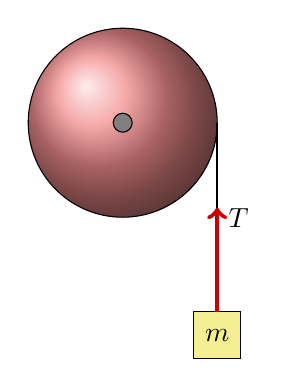
\begin{tikzpicture}[scale=.6]
      \tikzstyle{balloon}=[ball color=red!80!gray!50];
      \shade[balloon] (0,0) circle (2);% node[below right]{$m$};
      \draw(0,0) circle(2);
      \draw[fill=gray](0,0) circle(.2);
      \draw[thick](2,0)--(2,-4);
      \draw[fill=yellow!80!gray!50](1.5,-4) rectangle(2.5,-5)
      node[midway,black]{$m$};
      \draw[ultra thick,red!80!black,->](2,-4)--(2,-1.8)
      node[pos=.9,right,black]{$T$};
    \end{tikzpicture}
  \end{center}
  \begin{enumerate}[itemsep=1in,leftmargin=15pt]
  \item the acceleration of the body, and
  \item the tension in the string.
  \end{enumerate}
  \vspace{1in}
\item A uniform cylinder of mass $M$ and radius $R$ has a string wrapped around
  it. The string is held fixed, and the cylinder falls vertically as shown in
  the figure below. Find
  \begin{center}
    \vspace{-.3in}
    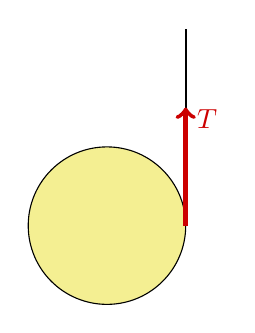
\begin{tikzpicture}[scale=.5]
      \draw[fill=yellow!80!gray!50](0,0) circle(2);
      \draw[thick](2,0)--(2,5);
%      \draw[fill=yellow!80!gray!50](1.5,-4) rectangle(2.5,-5)
%      node[midway,black]{$m$};
      \draw[ultra thick,red!80!black,->](2,0)--(2,3) node[pos=.9,right]{$T$};
    \end{tikzpicture}
  \end{center}
  \begin{enumerate}[itemsep=1in,leftmargin=15pt]
  \item\vspace{-.3in} the acceleration of the body, and
  \item the tension in the string.
  \end{enumerate}
  
%\item A mass $m$ is hung on a string that is wrapped around a disk of radius
%  $R$ and rotational inertia $I$. The mass is released from rest and
%  accelerates downward with an acceleration $a$.
%  \begin{enumerate}[noitemsep]
%  \item Determine the tension in the string as the mass accelerates downward
%    in terms of the given quantities.
%  \item In terms of the tension $T$ and the other given quantities, determine
%    the rate of change of the angular speed of the disk.
%  \end{enumerate}
%  \pic{.3}{mass-disk.png}
%  \vspace{.5in}
%  
%\item A disk having a rotational inertia of \SI{2.}{\kilo\gram.\metre^2}
%  rotates about a fixed axis through its center. The disk begins from rest at
%  $t=0$, and at time $t=\SI{2}{\second}$, its angular velocity is \SI{2}{rad\per\second}.
%  \begin{enumerate}[noitemsep]
%  \item Determine the angular momentum of the disk at $t=\SI{2}{\second}$.
%  \item What is the angular acceleration of the disk between $t=0$ and
%    $t=\SI{2}{\second}$?
%  \item What is the kinetic energy of the disk at $t=\SI{2}{\second}$?
%  \end{enumerate}
%  \pic{.3}{rotDisk.png}
  \newpage
%\item A mass $m$ oscillates on an ideal spring of spring constant $k$ on a
%  frictionless horizontal surface. The mass is pulled aside to a distance $A$
%  from its equilibrium position, and released.
%  \begin{center}
%    \begin{tikzpicture}
%      \fill [pattern=north east lines] (5,0)--(0,0)--(0,2)--(-0.2,2)
%      --(-0.2,-0.2)--(5,-0.2)--cycle;
%      \draw[ultra thick] (5,0)--(0,0)--(0,2)--(-0.5,2);
%      \draw[decoration={aspect=0.3,segment length=2mm, amplitude=2.5mm, coil},
%        decorate] (0,0.5)--(1.5,0.5);
%      \draw[fill=gray!70](1.5,0) rectangle(2.5,1);
%      \draw[thick](2.5,0)--(2.5,-0.3) node[pos=1,below]{O};
%      \draw[thick](4,0)--(4,-0.3) node[pos=1,below]{A};
%    \end{tikzpicture}
%  \end{center} 
%  \begin{enumerate}[noitemsep]  
%  \item In terms of the given quantities, at what distance from the equilibrium
%    position is the potential energy of the mass equal to its kinetic energy?
%  \item In terms of the given quantities, what is the acceleration of the mass
%    when it is at the amplitude $A$?
%  \end{enumerate}
%%  \vspace{3in}
%  \newpage
%  
%\item A mass oscillates in simple harmonic motion as shown by the position $x$
%  vs. time $t$ graph below.
%  \begin{center}
%    \pic{.45}{oscillate.png}
%  \end{center}
%  \begin{enumerate}[noitemsep]  
%  \item What is the frequency of oscillation?
%  \item Write the equation that represents the speed of the mass as a function
%    of time.
%  \end{enumerate}
%  \newpage

\item In heavy seas, the bow of a battle ship undergoes a simple harmonic
  vertical pitching motion with a period of \SI{8.}{\second} and an amplitude
  of \SI{2.}{\metre}.
  \begin{enumerate}[itemsep=.8in,topsep=0pt,leftmargin=15pt]
  \item What is the maximum vertical velocity of the battle ship's bow?
  \item What is its maximum acceleration?
  \item An \SI{80}{\kilo\gram} sailor is standing on the scale in the bunk room
    in the bow. What are the maximum and minimum reading on the scale in
    newtons?
    \vspace{.8in}
  \end{enumerate}

\item Show that for the situations in the figures below, the object of mass
  $m$ oscillates with a frequency of
  $\displaystyle f=\frac{1}{2\pi}\sqrt{\frac{k_\mathrm{eff}}{m}}$
  where $k_\mathrm{eff}$ is given by (a) $k_\mathrm{eff}=k_1+k_2$ and (b)
  $\displaystyle\frac{1}{k_\mathrm{eff}}=\frac{1}{k_1}+\frac{1}{k_2}$. Hint:
  find the net force on the mass and write $F=-k_\mathrm{eff}x$. Note that in
  (b), the springs stretch by different amounts, the sum of which is $x$.
  
  (a)\hspace{5pt}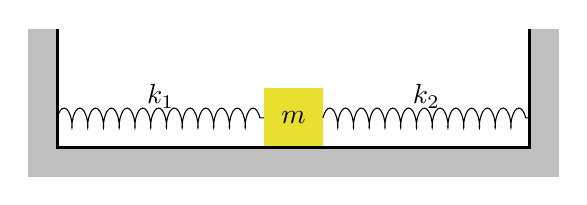
\begin{tikzpicture}[scale=.5]
    \fill[gray!50](0,0) rectangle(12,-.75);
    \fill[gray!50](-.75,-.75) rectangle(0,3);
    \fill[gray!50](12,-.75) rectangle(12.75,3);
    \fill[yellow!80!gray](5.25,0) rectangle(6.75,1.5) node[midway,black]{$m$};
    \draw[decoration={aspect=0.3,segment length=2mm, amplitude=1.25mm, coil},
      decorate] (0,.75)--(5.25,.75) node[midway,above]{$k_1$};
    \draw[decoration={aspect=0.3,segment length=2mm, amplitude=1.25mm, coil},
      decorate] (6.75,.75)--(12,.75) node[midway,above]{$k_2$};
    \draw[very thick](0,3)--(0,0)--(12,0)--(12,3);
  \end{tikzpicture}

  (b)\hspace{5pt}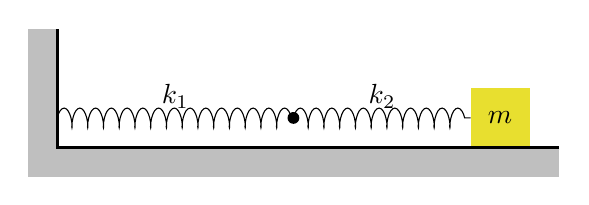
\begin{tikzpicture}[scale=.5]
    \fill[gray!50](0,0) rectangle(12.75,-.75);
    \fill[gray!50](-.75,-.75) rectangle(0,3);
    \fill[yellow!80!gray](10.5,0) rectangle(12,1.5) node[midway,black]{$m$};
    \draw[decoration={aspect=0.3,segment length=2mm, amplitude=1.25mm, coil},
      decorate] (0,.75)--(6,.75) node[midway,above]{$k_1$};
    \draw[decoration={aspect=0.3,segment length=2mm, amplitude=1.25mm, coil},
      decorate] (6,.75)--(10.5,.75) node[midway,above]{$k_2$};
    \fill[black](6,.75) circle(.15);
    \draw[very thick](0,3)--(0,0)--(12.75,0);
  \end{tikzpicture}
  \vspace{3in}
  
\item A simple pendulum of length $L$ is released from rest from an angle of
  $\theta_0$.
  \begin{enumerate}[itemsep=.8in,topsep=0pt,leftmargin=15pt]
  \item Assuming the motion of the pendulum to be simple harmonic motion, find
    its speed as it passes through $\theta=0$.
  \item Using the conservation of energy, find this speed exactly.
  \item Show that your results for (a) and (b) are the same when $\theta_0$ is
    small.
  \item Find the difference in your results for $\theta_0=\SI{.20}{rad}$ and
    $L=\SI{1}{\metre}$.
  \end{enumerate}
 
\end{enumerate}
\end{document}
